\documentclass[11pt,ignorenonframetext,]{beamer}
\setbeamertemplate{caption}[numbered]
\setbeamertemplate{caption label separator}{: }
\setbeamercolor{caption name}{fg=normal text.fg}
\beamertemplatenavigationsymbolsempty
\usepackage{lmodern}
\usepackage{amssymb,amsmath}
\usepackage{ifxetex,ifluatex}
\usepackage{fixltx2e} % provides \textsubscript
\ifnum 0\ifxetex 1\fi\ifluatex 1\fi=0 % if pdftex
  \usepackage[T1]{fontenc}
  \usepackage[utf8]{inputenc}
\else % if luatex or xelatex
  \ifxetex
    \usepackage{mathspec}
  \else
    \usepackage{fontspec}
  \fi
  \defaultfontfeatures{Ligatures=TeX,Scale=MatchLowercase}
\fi
\usetheme[]{metropolis}
% use upquote if available, for straight quotes in verbatim environments
\IfFileExists{upquote.sty}{\usepackage{upquote}}{}
% use microtype if available
\IfFileExists{microtype.sty}{%
\usepackage{microtype}
\UseMicrotypeSet[protrusion]{basicmath} % disable protrusion for tt fonts
}{}
\newif\ifbibliography
\hypersetup{
            pdftitle={Lecture 12},
            pdfauthor={Colin Rundel},
            pdfborder={0 0 0},
            breaklinks=true}
\urlstyle{same}  % don't use monospace font for urls
\usepackage{longtable,booktabs}
\usepackage{caption}
% These lines are needed to make table captions work with longtable:
\makeatletter
\def\fnum@table{\tablename~\thetable}
\makeatother
\usepackage{graphicx,grffile}
\makeatletter
\def\maxwidth{\ifdim\Gin@nat@width>\linewidth\linewidth\else\Gin@nat@width\fi}
\def\maxheight{\ifdim\Gin@nat@height>\textheight0.8\textheight\else\Gin@nat@height\fi}
\makeatother
% Scale images if necessary, so that they will not overflow the page
% margins by default, and it is still possible to overwrite the defaults
% using explicit options in \includegraphics[width, height, ...]{}
\setkeys{Gin}{width=\maxwidth,height=\maxheight,keepaspectratio}

% Prevent slide breaks in the middle of a paragraph:
\widowpenalties 1 10000
\raggedbottom

\AtBeginPart{
  \let\insertpartnumber\relax
  \let\partname\relax
  \frame{\partpage}
}
\AtBeginSection{
  \ifbibliography
  \else
    \let\insertsectionnumber\relax
    \let\sectionname\relax
    \frame{\sectionpage}
  \fi
}
\AtBeginSubsection{
  \let\insertsubsectionnumber\relax
  \let\subsectionname\relax
  \frame{\subsectionpage}
}

\setlength{\parindent}{0pt}
\setlength{\parskip}{6pt plus 2pt minus 1pt}
\setlength{\emergencystretch}{3em}  % prevent overfull lines
\providecommand{\tightlist}{%
  \setlength{\itemsep}{0pt}\setlength{\parskip}{0pt}}
\setcounter{secnumdepth}{0}

\usepackage{geometry}
\usepackage{graphicx}
\usepackage{amssymb}
\usepackage{color}          	% gives color options
\usepackage{url}		% produces hyperlinks
\usepackage[english]{babel}
\usepackage{colortbl}	% allows for color usage in tables
\usepackage{multirow}	% allows for rows that span multiple rows in tables
\usepackage{xcolor}		% this package has a variety of color options
\usepackage{calc}
\usepackage{multicol}
\usepackage{wrapfig}
\usepackage{textcomp}
\usepackage{bm}
\usepackage{bbm}
\usepackage{setspace}
\singlespacing

%%%%%%%%%%%%%%%%
% Small code output
%%%%%%%%%%%%%%%%

%% change fontsize of R code

\makeatletter
\@ifundefined{Shaded}{\newenvironment{Shaded}{}{}}{}
\makeatother


\let\oldShaded\Shaded
\let\endoldShaded\endShaded
\renewenvironment{Shaded}{\footnotesize\begin{spacing}{0.9}\oldShaded}{\endoldShaded\end{spacing}}

%% change fontsize of output
\let\oldverbatim\verbatim
\let\endoldverbatim\endverbatim
\renewenvironment{verbatim}{\footnotesize\begin{spacing}{0.9}\oldverbatim}{\endoldverbatim\end{spacing}}


\newcommand{\tinyoutput}{
  \renewenvironment{Shaded}{\tiny\begin{spacing}{0.9}\oldShaded}{\endoldShaded\end{spacing}}
  \renewenvironment{verbatim}{\tiny\begin{spacing}{0.9}\oldverbatim}{\endoldverbatim\end{spacing}}
}

\newcommand{\scriptoutput}{
  \renewenvironment{Shaded}{\scriptsize\begin{spacing}{0.9}\oldShaded}{\endoldShaded\end{spacing}}
  \renewenvironment{verbatim}{\scriptsize\begin{spacing}{0.9}\oldverbatim}{\endoldverbatim\end{spacing}}
}

\newcommand{\footnoteoutput}{
  \renewenvironment{Shaded}{\footnotesize\begin{spacing}{0.9}\oldShaded}{\endoldShaded\end{spacing}}
  \renewenvironment{verbatim}{\footnotesize\begin{spacing}{0.9}\oldverbatim}{\endoldverbatim\end{spacing}}
}

%\newcommand{\verbatimfont}[1]{\renewcommand{\verbatim@font}{\ttfamily#1}}


%%%%%%%%%%%%%%%%
% Custom Colors
%%%%%%%%%%%%%%%%

\xdefinecolor{oiBlue}{rgb}{0.15, 0.35, 0.55}
\xdefinecolor{gray}{rgb}{0.5, 0.5, 0.5}
\xdefinecolor{darkGray}{rgb}{0.3, 0.3, 0.3}
\xdefinecolor{darkerGray}{rgb}{0.2, 0.2, 0.2}
\xdefinecolor{rubineRed}{rgb}{0.89,0,0.30}
\xdefinecolor{linkCol}{rgb}{0.11,0.49,0.95}	
\xdefinecolor{irishGreen}{rgb}{0,0.60,0}	
\xdefinecolor{darkturquoise}{rgb}{0.44, 0.58, 0.86}
\definecolor{lightGreen}{rgb}{0.533,0.765,0.42}
%\xdefinecolor{hlblue}{rgb}{0.051,0.65,1}
\xdefinecolor{hlblue}{rgb}{ 0.055, 0.639, 0.831}
\definecolor{light}{rgb}{.337,.608,.741}
\definecolor{dark}{rgb}{.337,.608,.741}

\definecolor{cpink}{rgb}{0.93, 0.23, 0.51}

%%%%%%%%%%%%%%%%
% Custom Commands
%%%%%%%%%%%%%%%%

% text colors
\newcommand{\red}[1]{\textit{\textcolor{rubineRed}{#1}}}
\newcommand{\orange}[1]{\textit{\textcolor{orange}{#1}}}
\newcommand{\pink}[1]{\textit{\textcolor{rubineRed!90!white!50}{#1}}}
\newcommand{\green}[1]{\textit{\textcolor{irishGreen}{#1}}}
\newcommand{\blue}[1]{\textit{\textcolor{darkturquoise}{#1}}}
\newcommand{\light}[1]{\textcolor{light}{\textbf{#1}}}
\newcommand{\dark}[1]{\textcolor{dark}{#1}}
\newcommand{\gray}[1]{\textcolor{gray}{#1}}


% links: webURL, webLin, appLink
\newcommand{\webURL}[1]{\urlstyle{same}{\textit{\textcolor{linkCol}{\url{#1}}} }}
\newcommand{\webLink}[2]{\href{#1}{\textcolor{linkCol}{{#2}}}}
\newcommand{\appLink}[2]{\href{#1}{\textcolor{lightGreen!80!black!90}{{#2}}}}

% mail
\newcommand{\mail}[1]{\href{mailto:#1}{\textit{\textcolor{linkCol}{#1}}}}

% highlighting: hl, hlGr, mathhl
\newcommand{\hl}[1]{\textit{\textcolor{hlblue}{#1}}}
\newcommand{\hlGr}[1]{\textit{\textcolor{lightGreen}{#1}}}
\newcommand{\hlRd}[1]{\textit{\textcolor{rubineRed}{#1}}}
\newcommand{\mathhl}[1]{\textcolor{hlblue}{\ensuremath{#1}}}

% example
\newcommand{\ex}[1]{\textcolor{blue}{{{\small (#1)}}}}


\DeclareMathOperator*{\argmin}{arg\,min}
\DeclareMathOperator*{\argmax}{arg\,max}

\title{Lecture 12}
\subtitle{Gaussian Process Models}
\author{Colin Rundel}
\date{02/27/2017}

\begin{document}
\frame{\titlepage}

\section{Multivariate Normal}\label{multivariate-normal}

\begin{frame}[t]{Multivariate Normal Distribution}

For an \(n\)-dimension multivate normal distribution with covariance
\(\bm{\Sigma}\) (positive semidefinite) can be written as

\[
\underset{n \times 1}{\bm{Y}} \sim N(\underset{n \times 1}{\bm{\mu}}, \; \underset{n \times n}{\bm{\Sigma}}) \text{   where   } \{\bm{\Sigma}\}_{ij} = \sigma^2_{ij} = \rho_{ij} \, \sigma_{i} \, \sigma_{j}
\]

\vspace{2mm}

\[
\begin{pmatrix}
Y_1\\ \vdots\\ Y_n
\end{pmatrix}
\sim N\left(
\begin{pmatrix}
\mu_1\\ \vdots\\ \mu_n
\end{pmatrix}, \,
\begin{pmatrix}
\rho_{11}\sigma_1\sigma_1 & \cdots & \rho_{1n}\sigma_1\sigma_n \\
\vdots & \ddots & \vdots \\
\rho_{n1}\sigma_n\sigma_1 & \cdots & \rho_{nn}\sigma_n\sigma_n \\
\end{pmatrix}
\right)
\]

\end{frame}

\begin{frame}[t]{Density}

For the \(n\) dimensional multivate normal given on the last slide, its
density is given by

\[
(2\pi)^{-n/2} \; \det(\bm{\Sigma})^{-1/2} \; \exp{\left(-\frac{1}{2} \underset{1 \times n}{(\bm{Y}-\bm{\mu})'} \underset{n \times n}{\bm{\Sigma}^{-1}} \underset{n \times 1}{(\bm{Y}-\bm{\mu})}\right)} 
\]

and its log density is given by

\[
-\frac{n}{2} \log 2\pi - \frac{1}{2} \log \det(\bm{\Sigma}) - -\frac{1}{2} \underset{1 \times n}{(\bm{Y}-\bm{\mu})'} \underset{n \times n}{\bm{\Sigma}^{-1}} \underset{n \times 1}{(\bm{Y}-\bm{\mu})}
\]

\end{frame}

\begin{frame}[t]{Sampling}

To generate draws from an \(n\)-dimensional multivate normal with mean
\(\bm\mu\) and covariance matrix \(\bm\Sigma\),

\vspace{4mm}

\pause

\begin{itemize}
\tightlist
\item
  Find a matrix \(\bm{A}\) such that \(\bm\Sigma = \bm{A}\,\bm{A}^t\),
  most often we use \(\bm{A} = \text{Chol}(\bm\Sigma)\)
\end{itemize}

\pause

\vspace{2mm}

\begin{itemize}
\tightlist
\item
  Draw \(n\) iid unit normals (\(\mathcal{N}(0,1)\)) as \(\bm{z}\)
\end{itemize}

\pause

\vspace{2mm}

\begin{itemize}
\tightlist
\item
  Construct multivariate normal draws using
  \[ \bm{Y} = \bm\mu + \bm{A} \, \bm{z} \]
\end{itemize}

\end{frame}

\begin{frame}{Bivariate Example}

\scriptsize
\[ \bm{\mu} = \begin{pmatrix}0 \\ 0\end{pmatrix} \qquad \bm{\Sigma} = \begin{pmatrix}1 & \rho \\ \rho & 1 \end{pmatrix}\]

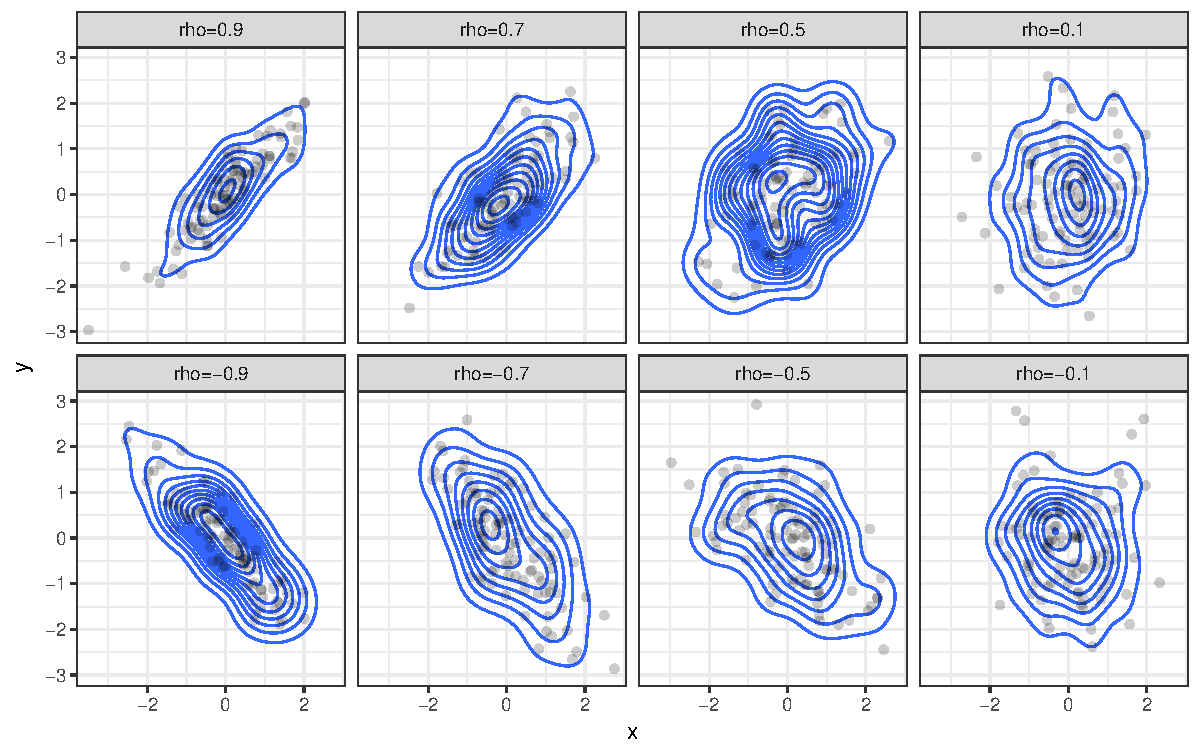
\includegraphics{Lec12_files/figure-beamer/unnamed-chunk-1-1.pdf}

\end{frame}

\begin{frame}{Marginal distributions}

\small

\textbf{Proposition} - For an \(n\)-dimensional multivate normal with
mean \(\bm\mu\) and covariance matrix \(\bm\Sigma\), any of the possible
marginal distributions will also (multivariate) normal.

\pause

\vspace{2mm}

For a univariate marginal distribution,
\[ y_i = \mathcal{N}(\mu_i,\,\gamma_{ii}) \]

\pause

For a bivariate marginal distribution,
\[ \bm{y}_{ij} = \mathcal{N}\left( \begin{pmatrix}\mu_i \\ \mu_j \end{pmatrix},\; \begin{pmatrix} \gamma_{ii} & \gamma_{ij} \\ \gamma_{ji} & \gamma_{jj} \end{pmatrix} \right) \]

\pause

For a \(k\)-dimensional marginal distribution,

\[ 
\bm{y}_{i_1,\cdots,i_k} = 
  \mathcal{N}\left( 
    \begin{pmatrix}\mu_{i_1} \\ \vdots \\ \mu_j \end{pmatrix},\; 
    \begin{pmatrix} 
      \gamma_{i_1i_1}  & \cdots & \gamma_{i_1 i_k} \\ 
      \vdots           & \ddots & \vdots \\
      \gamma_{i_k i_1} & \cdots & \gamma_{i_k i_k} \end{pmatrix} 
  \right) 
\]

\end{frame}

\begin{frame}[t]{Conditional Distributions}

If we partition the \(n\)-dimensions into two pieces such that
\(\bm{Y} = (\bm{Y}_1,\, \bm{Y}_2)^t\) then \footnotesize
\[
\underset{n \times 1}{\bm{Y}} \sim \mathcal{N}\left(
  \underset{n \times 1}{\begin{pmatrix}\bm{\mu}_1 \\ \bm{\mu}_2\end{pmatrix}},\, 
  \underset{n \times n}{\begin{pmatrix} 
    \bm{\Sigma}_{11} & \bm{\Sigma}_{12} \\ 
    \bm{\Sigma}_{21} & \bm{\Sigma}_{22} 
  \end{pmatrix}}
\right)
\] \[ \begin{aligned}
\underset{k \times 1}{\bm{Y}_1} &\sim \mathcal{N}(\underset{k \times 1}{\bm{\mu}_1},\, \underset{k \times k}{\bm{\Sigma}_{11}}) \\ 
\underset{n-k \times 1}{\bm{Y}_2} &\sim \mathcal{N}(\underset{n-k \times 1}{\bm{\mu}_2},\, \underset{n-k \times n-k}{\bm{\Sigma}_{22}})
\end{aligned} \]

\pause

\normalsize \vspace{2mm} then the conditional distributions are given by

\footnotesize
\[\begin{aligned}
\bm Y_1 ~|~ \bm{Y}_2 = \bm{a} ~&\sim \mathcal{N}(\bm\mu_1 + \bm\Sigma_{12} \, \bm\Sigma_{22}^{-1} \, (\bm{a} - \bm\mu_2),~ \bm\Sigma_{11}-\bm\Sigma_{12}\,\bm\Sigma_{22}^{-1} \, \bm\Sigma_{21}) \\
\\
\bm Y_2 ~|~ \bm{Y}_1 = \bm{b} ~&\sim \mathcal{N}(\bm\mu_2 + \bm\Sigma_{21} \, \bm\Sigma_{11}^{-1} \, (\bm{b} - \bm\mu_1),~ \bm\Sigma_{22}-\bm\Sigma_{21}\,\bm\Sigma_{11}^{-1} \, \bm\Sigma_{21})
\end{aligned}\]

\end{frame}

\begin{frame}[t]{Gaussian Processes}

From Shumway,

\begin{quote}
A process, \(\bm{Y} = \{Y_t ~:~ t \in T\}\), is said to be a Gaussian
process if all possible finite dimensional vectors
\(\bm{y} = (y_{t_1},y_{t_2},...,y_{t_n})^t\), for every collection of
time points \(t_1, t_2, \ldots , t_n\), and every positive integer
\(n\), have a multivariate normal distribution.
\end{quote}

\pause

So far we have only looked at examples of time series where \(T\) is
discete (and evenly spaces \& contiguous), it turns out things get a lot
more interesting when we explore the case where \(T\) is defined on a
\emph{continuous} space (e.g. \(\mathbb{R}\) or some subset of
\(\mathbb{R}\)).

\end{frame}

\section{Gaussian Process Regression}\label{gaussian-process-regression}

\begin{frame}[t]{Parameterizing a Gaussian Process}

Imagine we have a Gaussian process defined such that
\(\bm{Y} = \{Y_t ~:~ t \in [0,1]\}\),

\pause

\begin{itemize}
\tightlist
\item
  We now have an uncountably infinite set of possible \(Y_t\)s.
\end{itemize}

\pause

\begin{itemize}
\tightlist
\item
  We will only have a (small) finite number of observations
  \(Y_1, \ldots, Y_n\) with which to say something useful about this
  infinite dimension process.
\end{itemize}

\pause

\begin{itemize}
\tightlist
\item
  The unconstrained covariance matrix for the observed data can have up
  to \(n(n+1)/2\) unique values (\(p >>> n\))
\end{itemize}

\pause

\begin{itemize}
\item
  Necessary to make some simplifying assumptions:

  \begin{itemize}
  \item
    Stationarity
  \item
    Simple parameterization of \(\Sigma\)
  \end{itemize}
\end{itemize}

\end{frame}

\begin{frame}{Covariance Functions}

More on these next week, but for now some simple / common examples

Exponential Covariance:
\[ \Sigma(y_{t},y_{t'}) = \sigma^2 \exp\big(-|t-t'| \; l\,\big) \]

Squared Exponential Covariance:
\[ \Sigma(y_{t},y_{t'}) = \sigma^2 \exp\big(-(|t-t'| \; l\,)^2\big) \]

Powered Exponential Covariance (\(p \in (0,2]\)):
\[ \Sigma(y_{t},y_{t'}) = \sigma^2 \exp\big(-(|t-t'| \; l\,)^p\big) \]

\end{frame}

\begin{frame}{Covariance Function Decay}

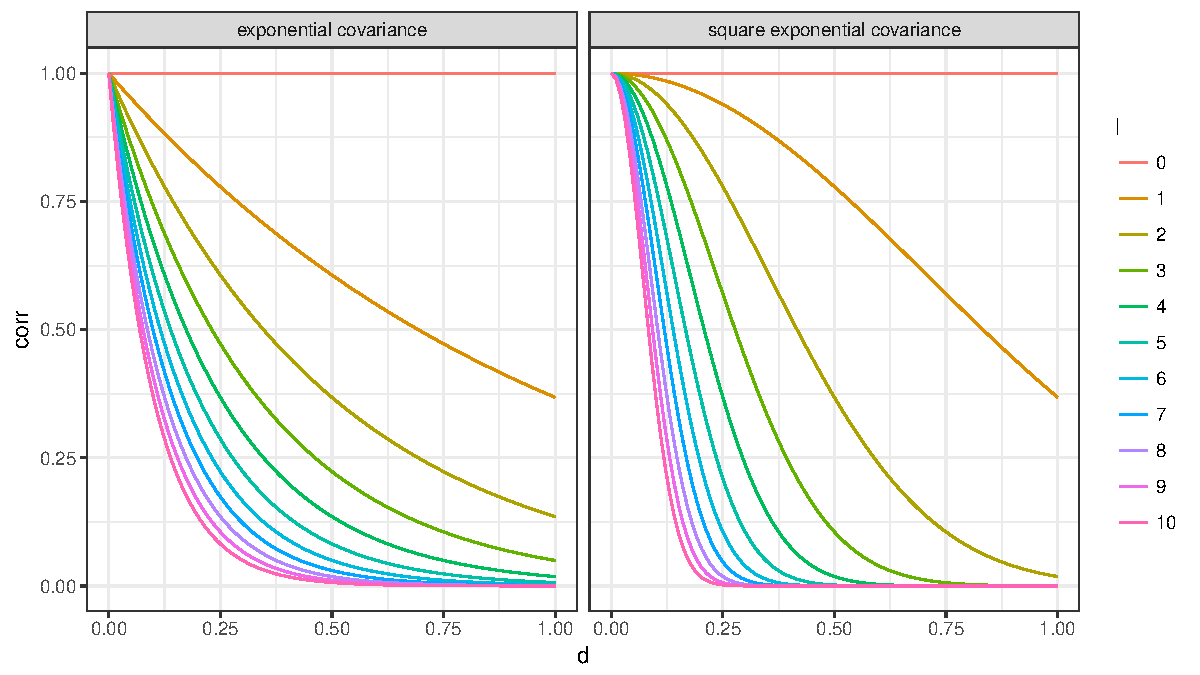
\includegraphics{Lec12_files/figure-beamer/unnamed-chunk-2-1.pdf}

\end{frame}

\begin{frame}{Example}

\begin{center}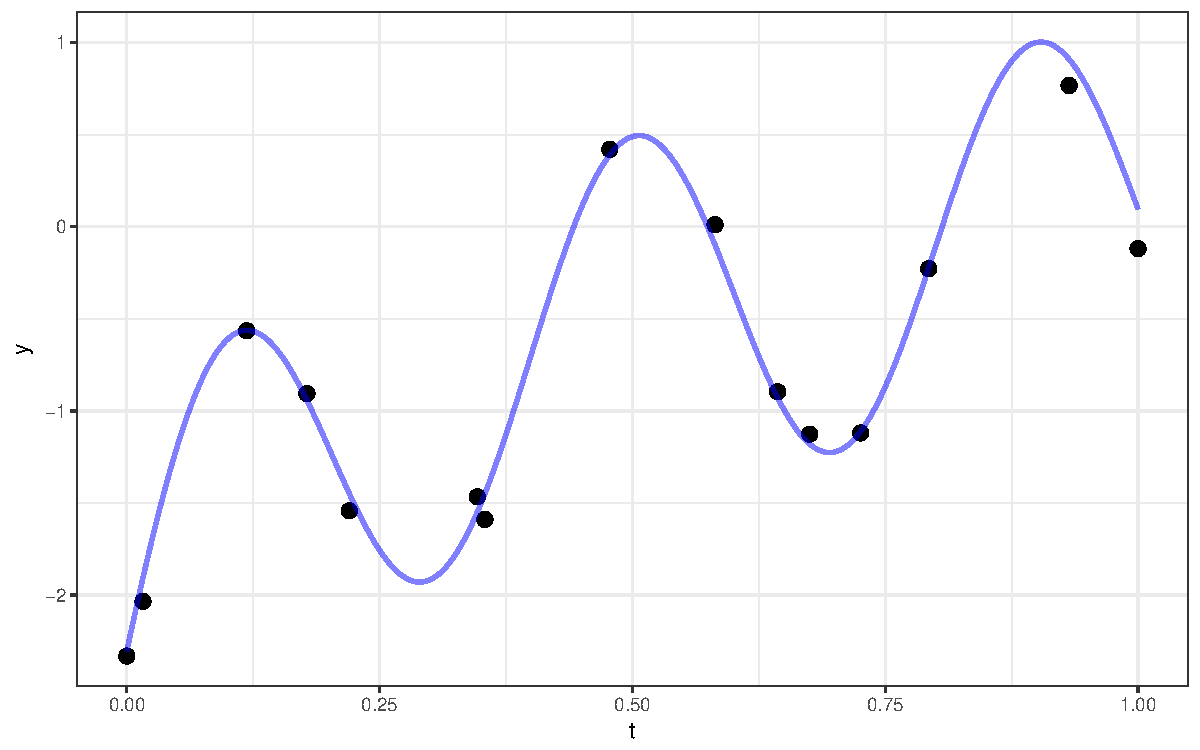
\includegraphics{Lec12_files/figure-beamer/unnamed-chunk-3-1} \end{center}

\end{frame}

\begin{frame}[t]{Prediction}

Our example has 15 observations which we would like to use as the basis
for predicting \(Y_t\) at other values of \(t\) (say a grid of values
from 0 to 1).

\vspace{3mm}

\pause

For now lets use a square exponential covariance with \(\sigma^2 = 10\)
and \(l=10\)

\vspace{3mm}

\pause

We therefore want to sample from \(\bm{Y}_{pred} | \bm{Y}_{obs}\).

\[\bm Y_{pred} ~|~ \bm{Y}_obs = \bm{y} ~\sim \mathcal{N}(\bm\Sigma_{po} \, \bm\Sigma_{obs}^{-1} \, \bm{y},~ \bm\Sigma_{pred}-\bm\Sigma_{po}\,\bm\Sigma_{pred}^{-1} \, \bm\Sigma_{op})\]

\end{frame}

\begin{frame}{Draw 1}

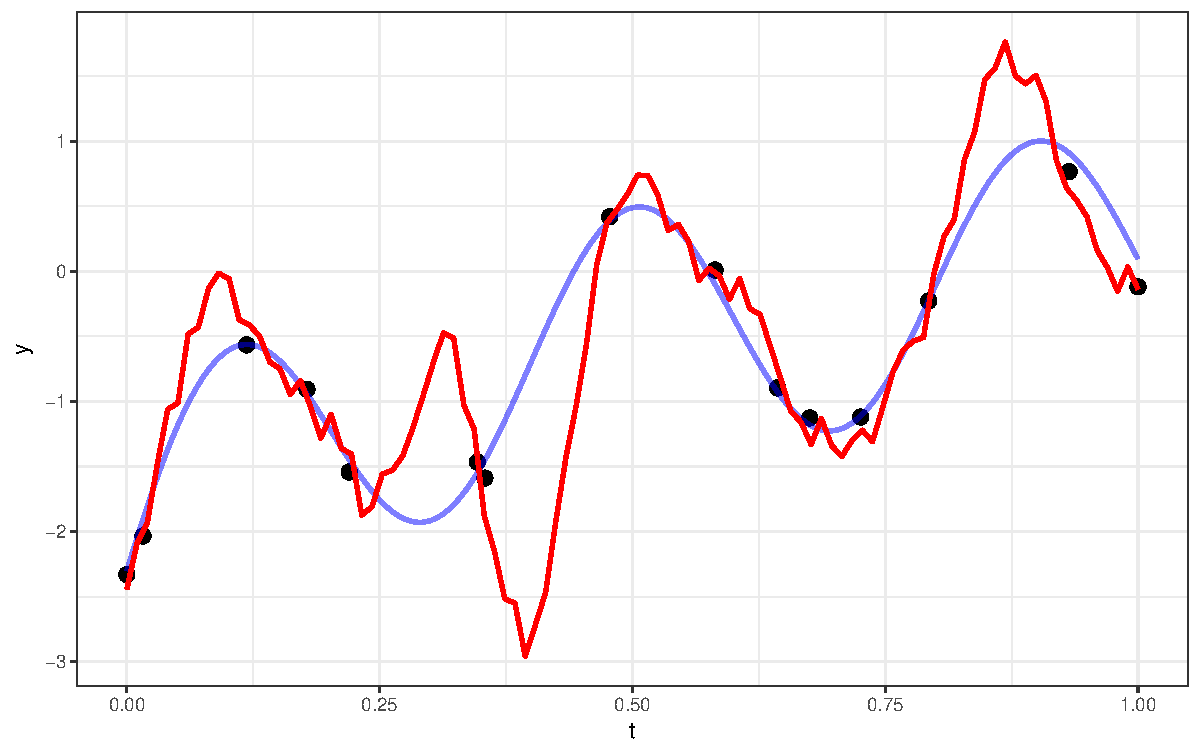
\includegraphics{Lec12_files/figure-beamer/unnamed-chunk-5-1.pdf}

\end{frame}

\begin{frame}{Draw 2}

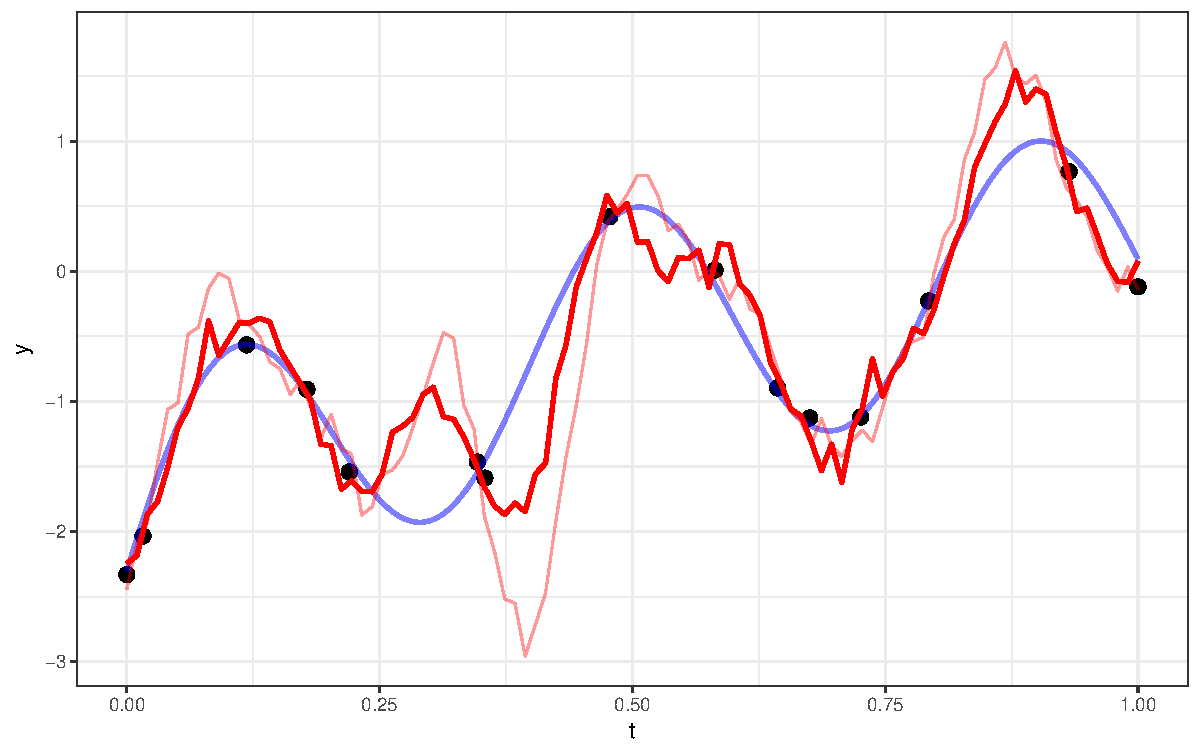
\includegraphics{Lec12_files/figure-beamer/unnamed-chunk-6-1.pdf}

\end{frame}

\begin{frame}{Draw 3}

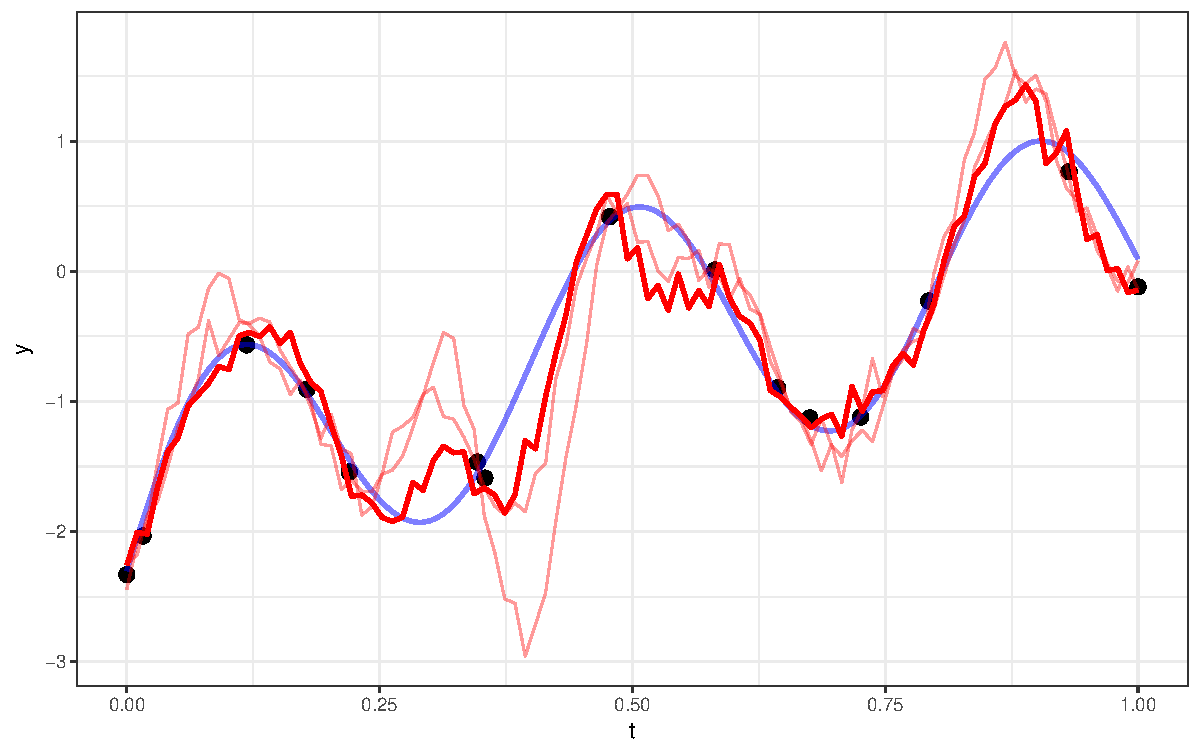
\includegraphics{Lec12_files/figure-beamer/unnamed-chunk-7-1.pdf}

\end{frame}

\begin{frame}{Draw 4}

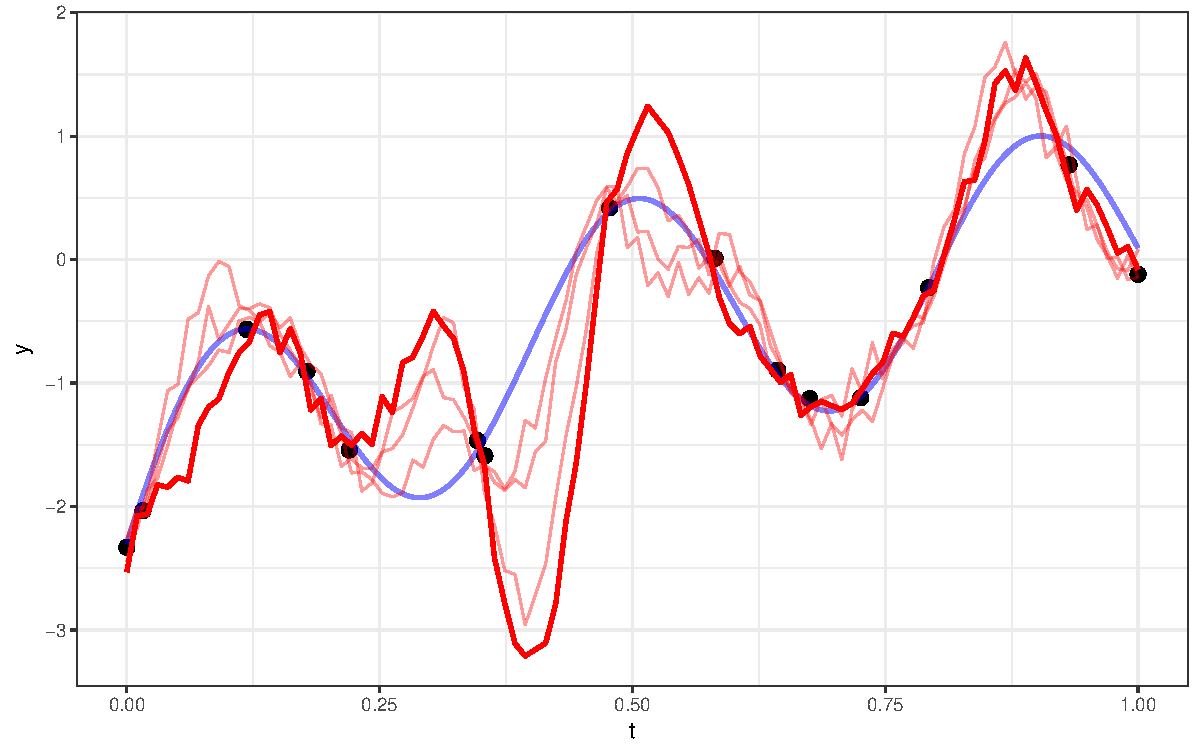
\includegraphics{Lec12_files/figure-beamer/unnamed-chunk-8-1.pdf}

\end{frame}

\begin{frame}{Draw 5}

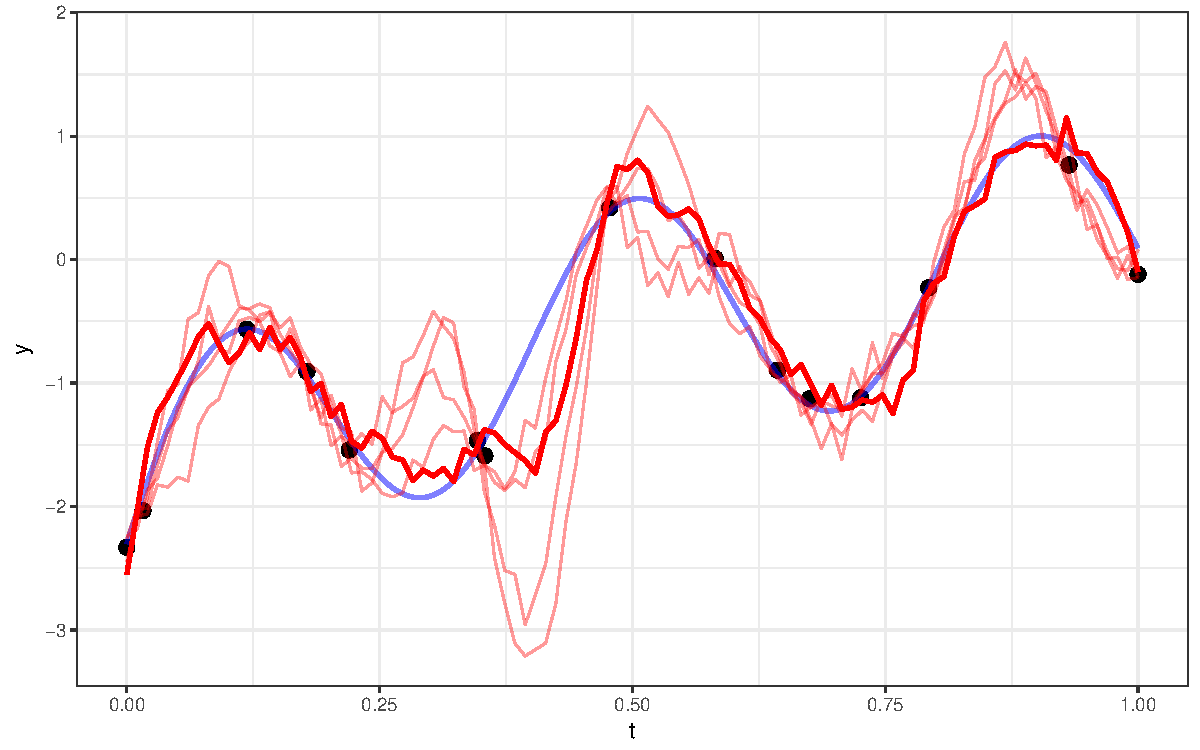
\includegraphics{Lec12_files/figure-beamer/unnamed-chunk-9-1.pdf}

\end{frame}

\begin{frame}{Many draws later}

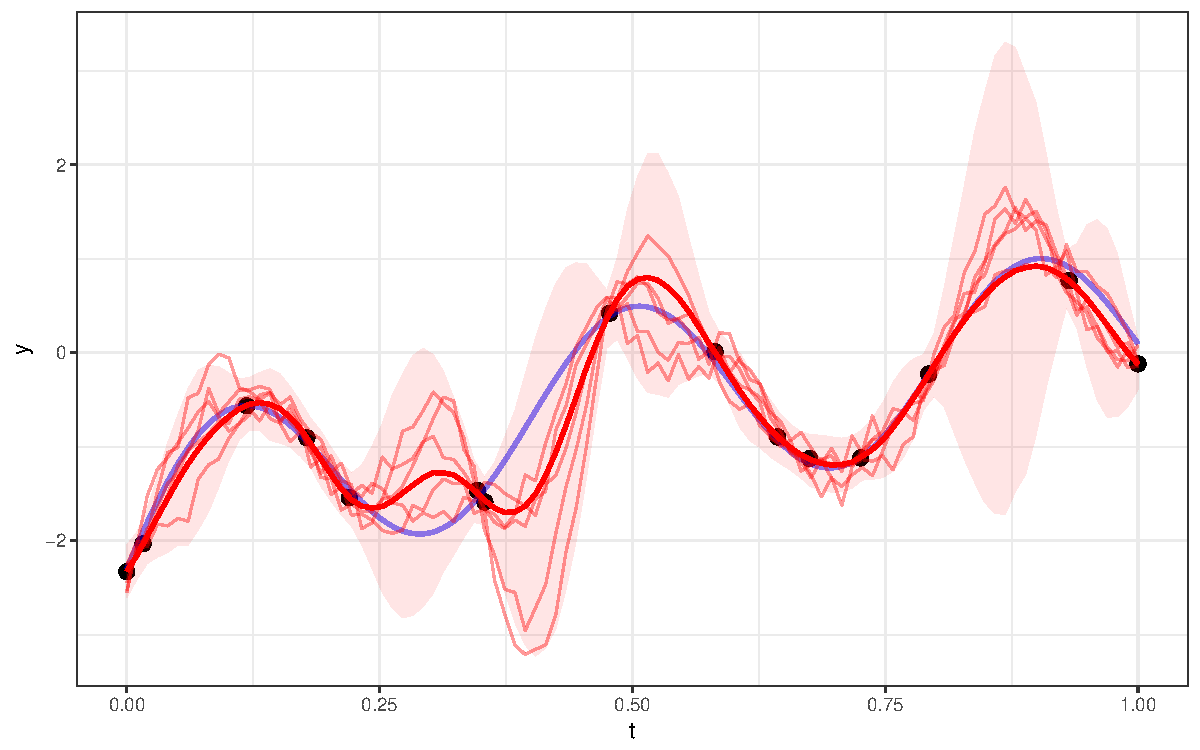
\includegraphics{Lec12_files/figure-beamer/unnamed-chunk-10-1.pdf}

\end{frame}

\begin{frame}{Exponential Covariance}

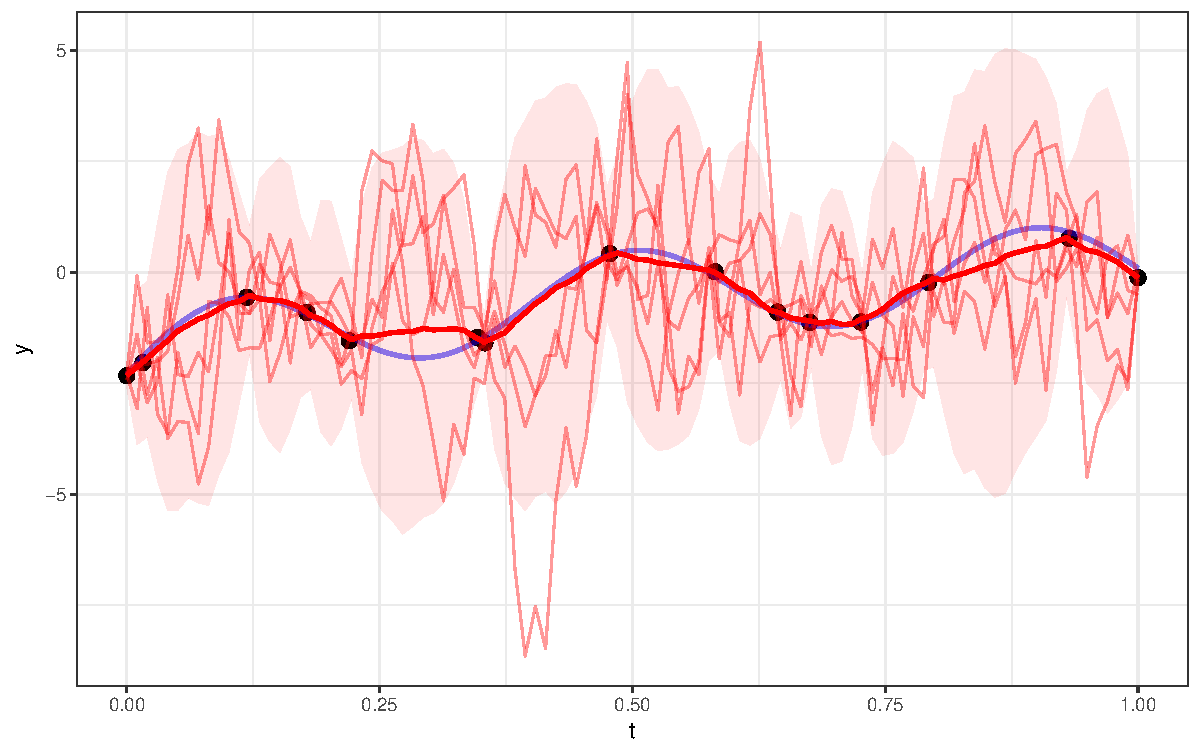
\includegraphics{Lec12_files/figure-beamer/unnamed-chunk-11-1.pdf}

\end{frame}

\begin{frame}{Powered Exponential Covariance (\(p=1.5\))}

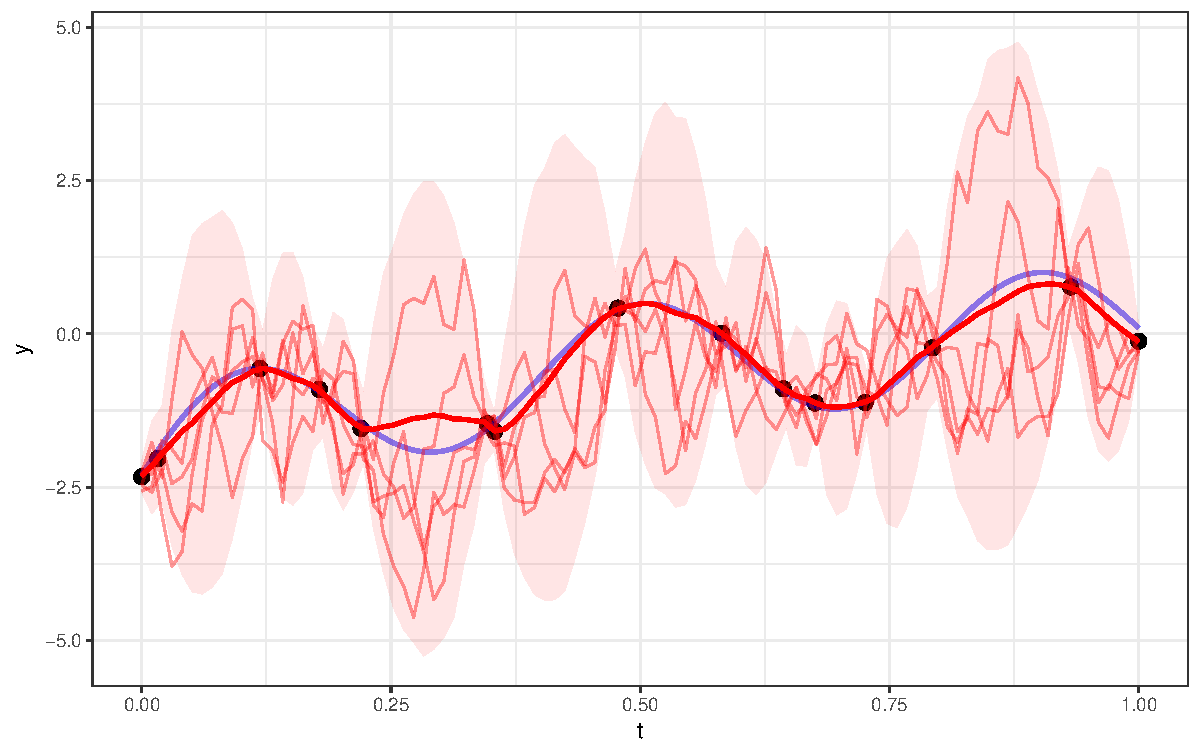
\includegraphics{Lec12_files/figure-beamer/unnamed-chunk-12-1.pdf}

\end{frame}

\begin{frame}{Back to the square exponential}

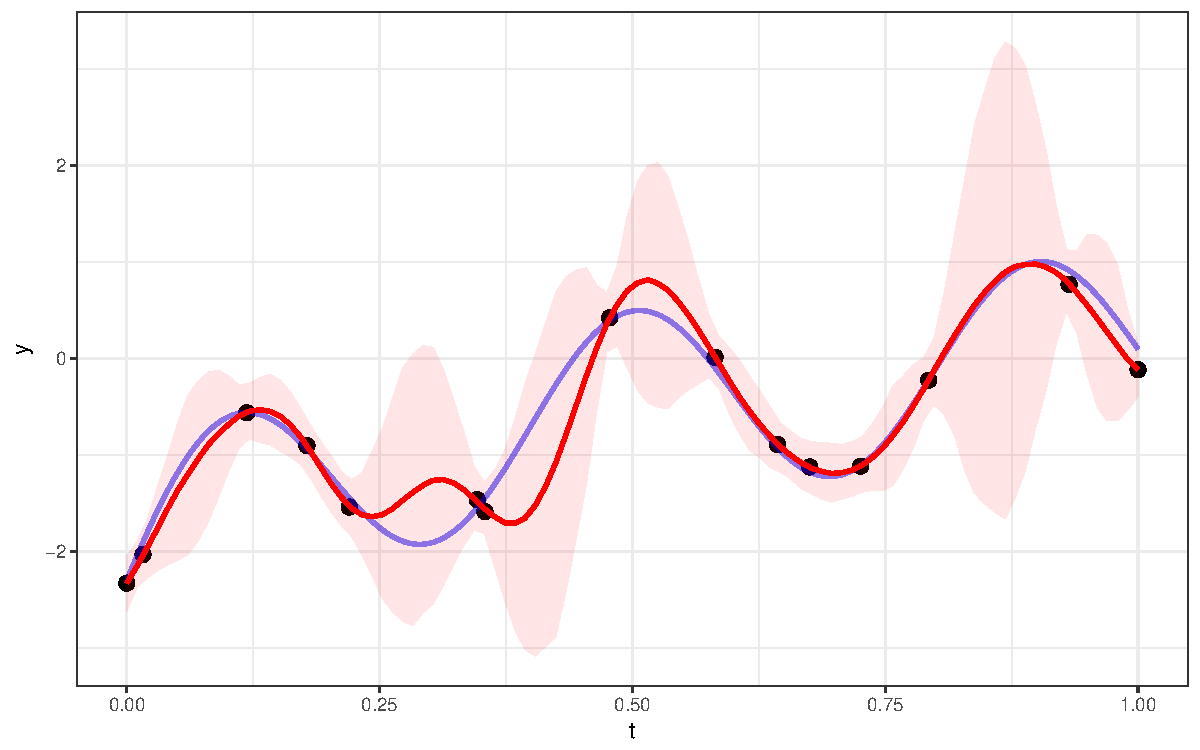
\includegraphics{Lec12_files/figure-beamer/unnamed-chunk-13-1.pdf}

\end{frame}

\begin{frame}{Changing the range (\(l\))}

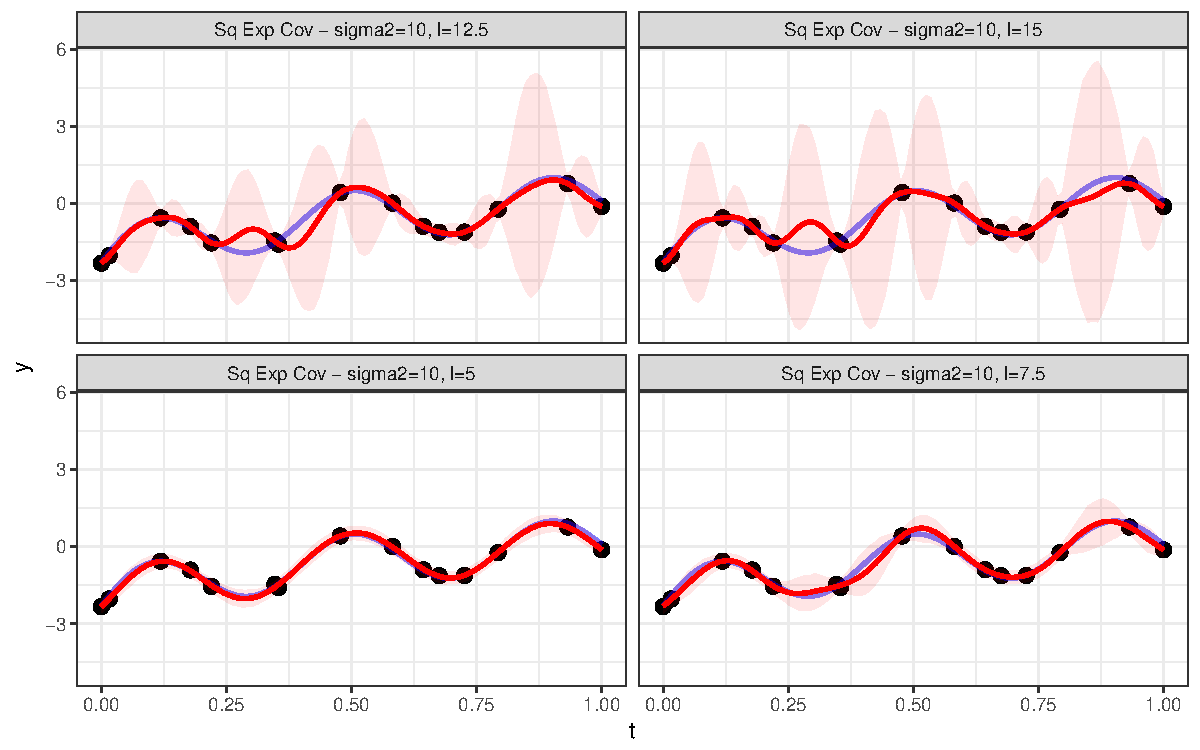
\includegraphics{Lec12_files/figure-beamer/unnamed-chunk-14-1.pdf}

\end{frame}

\begin{frame}[t]{Effective Range}

For the square exponential covariance \[ \begin{aligned} 
Cov(d) &= \sigma^2 \exp\left(-(l \cdot d)^2\right) \\
Corr(d) &= \exp\left(-(l \cdot d)^2\right)
\end{aligned} \]

we would like to know, for a given value of \(l\), beyond what distance
apart must observations be to have a correlation less than \(0.05\)?

\end{frame}

\begin{frame}{Changing the scale (\(\sigma^2\))}

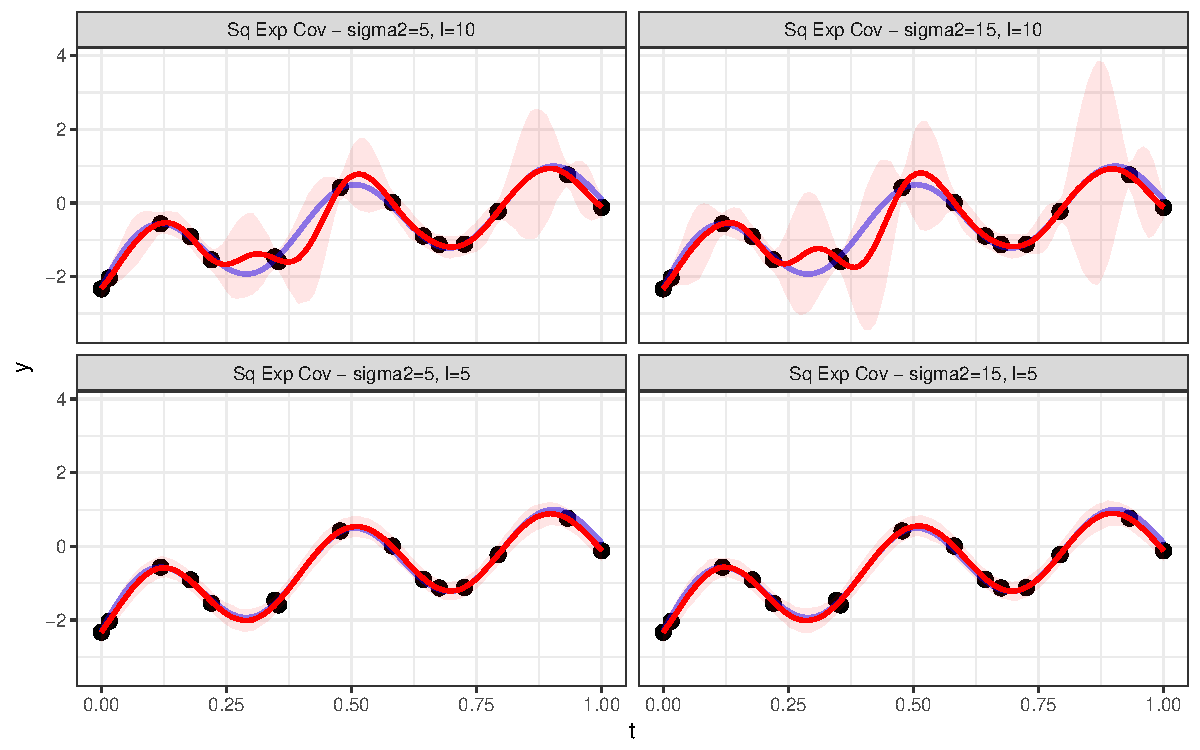
\includegraphics{Lec12_files/figure-beamer/unnamed-chunk-15-1.pdf}

\end{frame}

\begin{frame}[fragile]{Fitting}

\begin{verbatim}
## model{
##   y ~ dmnorm(mu, inverse(Sigma))
## 
##   for (i in 1:N) {
##     mu[i] <- 0
##   }
## 
##   for (i in 1:(N-1)) {
##     for (j in (i+1):N) {
##       Sigma[i,j] <- sigma2 * exp(- pow(l*d[i,j],2))
##       Sigma[j,i] <- Sigma[i,j]
##     }
##   }
## 
##   for (k in 1:N) {
##     Sigma[k,k] <- sigma2 + 0.01
##   }
## 
##   sigma2   ~ dlnorm(0, 1)
##   l        ~ dt(0, 2.5, 1) T(0,) # Half-cauchy(0,2.5)
## }
\end{verbatim}

\end{frame}

\begin{frame}{Trace plots}

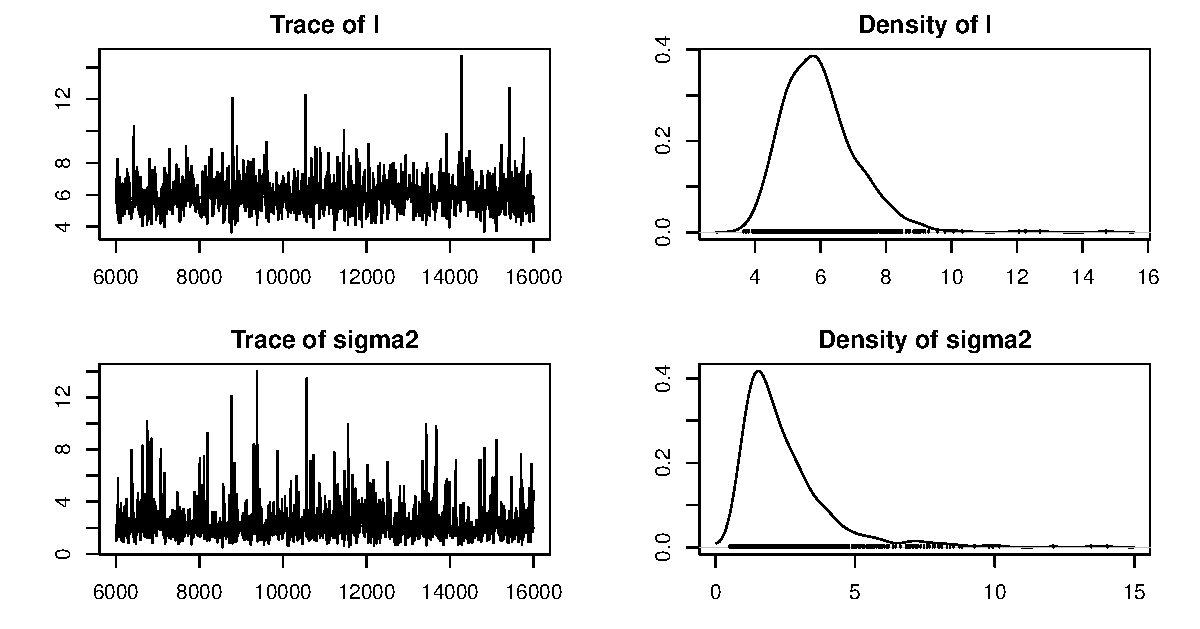
\includegraphics{Lec12_files/figure-beamer/unnamed-chunk-18-1.pdf}

\footnotesize

\begin{longtable}[]{@{}lrrrr@{}}
\toprule
param & post\_mean & post\_med & post\_lower &
post\_upper\tabularnewline
\midrule
\endhead
l & 5.981289 & 5.833655 & 4.2669795 & 8.456006\tabularnewline
sigma2 & 2.457979 & 2.032632 & 0.8173064 & 7.168197\tabularnewline
\bottomrule
\end{longtable}

\end{frame}

\begin{frame}{Fitted models}

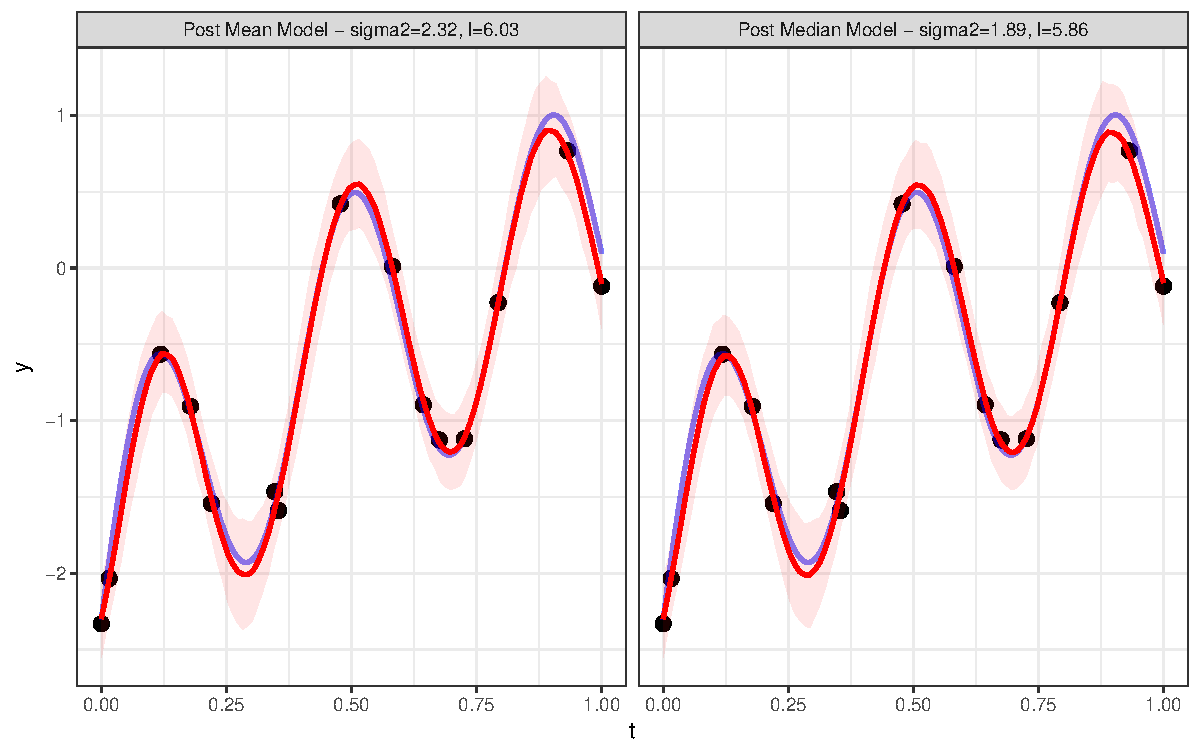
\includegraphics{Lec12_files/figure-beamer/unnamed-chunk-20-1.pdf}

\end{frame}

\begin{frame}{Forcasting}

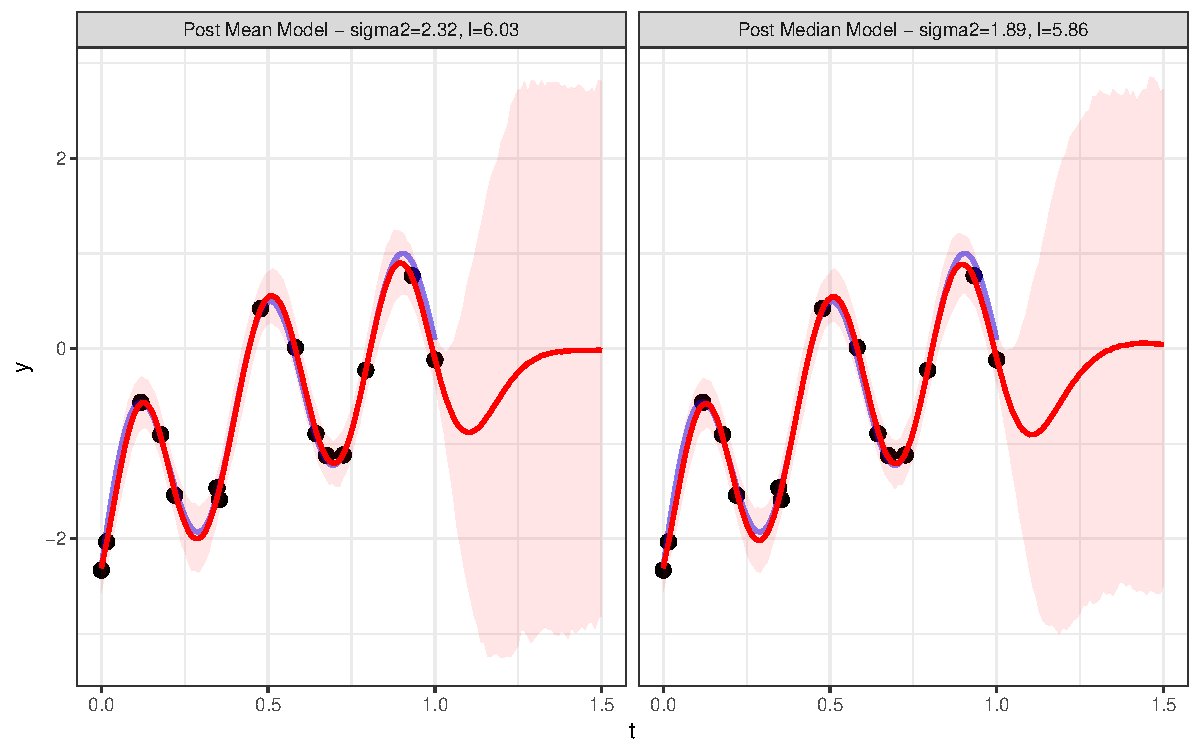
\includegraphics{Lec12_files/figure-beamer/unnamed-chunk-21-1.pdf}

\end{frame}

\end{document}
